\documentclass[border=10pt]{standalone}

\usepackage{tikz}
\usepackage{tikzsymbols}
\usetikzlibrary{calc,patterns,shapes.geometric}

\def\centerarc[#1](#2)(#3:#4:#5){\draw[#1] ($(#2)+({#5*cos(#3)},{#5*sin(#3)})$) arc (#3:#4:#5);}

\begin{document}
	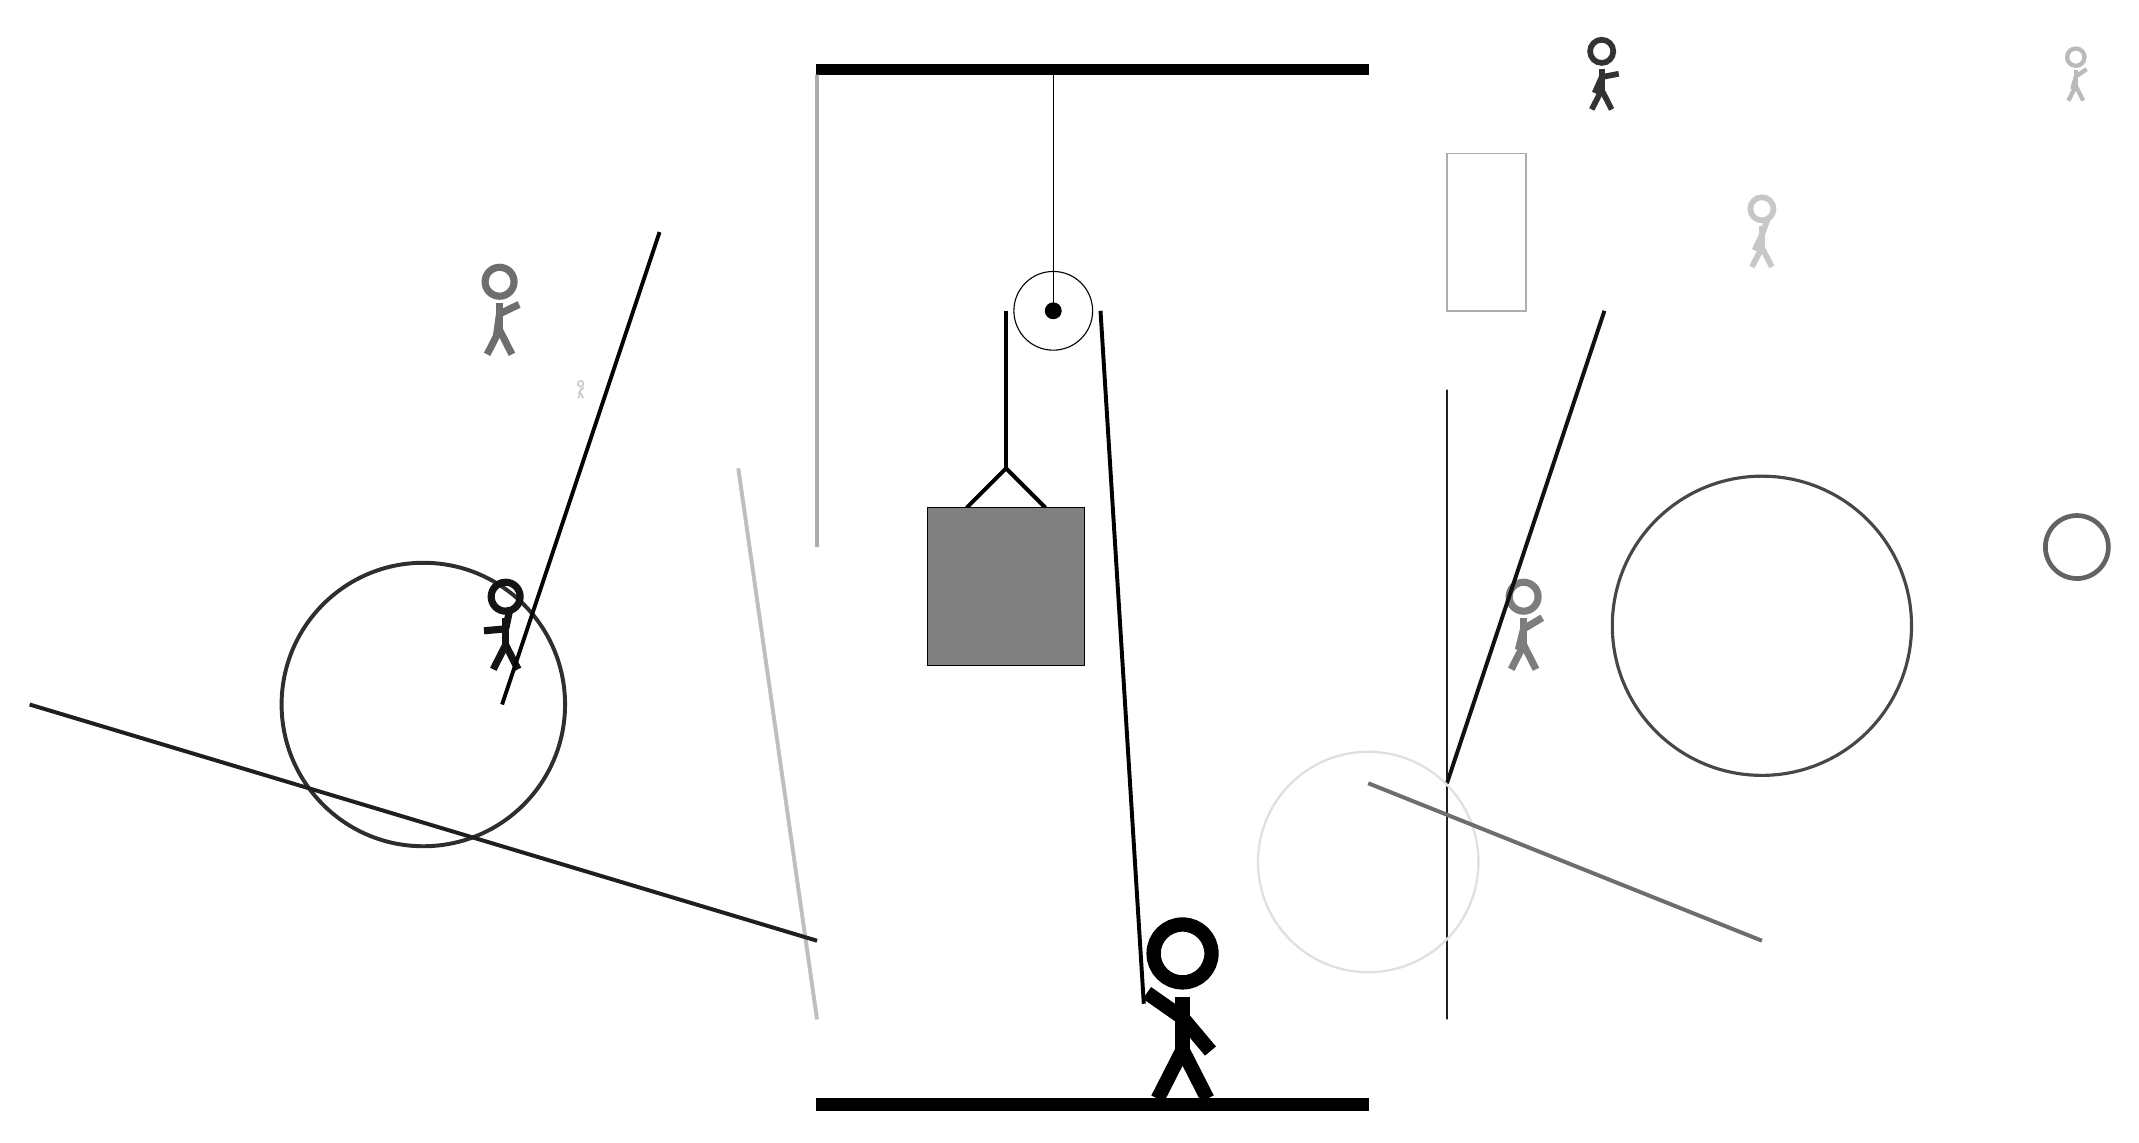
\begin{tikzpicture}
		%%%%% START %%%%%
		
		\draw[fill=black] (-2, 10) rectangle (5, 10.125);
		
		\draw (1, 7) circle (0.5);
		\draw[fill=black] (1, 7) circle (0.1);
		\draw (1, 10) -- (1, 7);
		
		\draw[line width=0.5mm] (-0.1, 4.5) -- (0.4, 5.0) -- (0.9, 4.5);
		\draw[fill=black!50] (-0.6, 4.5) rectangle (1.4, 2.5);
		
		\draw[line width=0.5mm] (0.4, 7) -- (0.4, 5.0);
		\centerarc[line width=0.5mm](1, 7)(0:180:0.6);
		\draw[line width=0.5mm](1.6, 7) -- (2.15, -1.8);
		
		\node[line width=0.6mm, color=black!80] at (8, 10) {\Strichmaxerl[4][66][11]};
		
		\draw [line width=0.5mm, color=black!82](-7, 2) circle (1.8);
		\draw[line width=0.5mm, color=black!25](-2, -2) -- (-3, 5);
		\draw [line width=0.4mm, color=black!72](10, 3) circle (1.9);
		\node[line width=0.2mm, color=black!51] at (7, 3) {\Strichmaxerl[5][76][31]};
		\draw [line width=0.6mm, color=black!61](14, 4) circle (0.4);
		\draw[line width=0.3mm, color=black!88] (6, -2) rectangle (6, 6);
		
		\node[line width=0.3mm, color=black!57] at (-6, 7) {\Strichmaxerl[5][82][26]};
		\draw[line width=0.5mm, color=black!88](-2, -1) -- (-12, 2);
		\draw[line width=0.5mm, color=black!93](8, 7) -- (6, 1);
		\draw [line width=0.3mm, color=black!12](5, 0) circle (1.4);
		\draw[line width=0.2mm, color=black!32] (6, 9) rectangle (7, 7);
		\draw[line width=0.6mm, color=black!32] (-2, 10) rectangle (-2, 4);
		\draw[line width=0.5mm, color=black!57](10, -1) -- (5, 1);
		\node[line width=0.5mm, color=black!22] at (10, 8) {\Strichmaxerl[4][65][69]};
		\node[line width=0.4mm, color=black!92] at (-6, 3) {\Strichmaxerl[5][5][78]};
		
		\node[line width=0.5mm, color=black!27] at (14, 10) {\Strichmaxerl[3][74][34]};
		\draw[line width=0.5mm, color=black!98](-6, 2) -- (-4, 8);
		\node[line width=0.2mm, color=black!22] at (-5, 6) {\Strichmaxerl[1][62][41]};
		
		
		\node at (2.6, -1.9) {\Strichmaxerl[10][-35][-50]};
		
		\draw[fill=black] (-2, -3) rectangle (5, -3.15);
		
		%%%%% END %%%%%
	\end{tikzpicture}
\end{document}